\section{Related Work}
\label{sec:related_work}
%\hongyi{Move the stuff about USB protocol to Background}\\
%\outline{Attack based on USB 1.0, briefly}\\
%\outline{Attack based on USB 2.0, focus on works about application and transport layer}\\
%\outline{Attack survey table}\\
%\outline{Attack or current works about USB Type-C}\\

We survey related works on USB attacks in Section~\ref{subsec:usb_attack} and
USB security defense in Section~\ref{subsec:usb_defence}, respectively.

\subsection{USB Attacks}
\label{subsec:usb_attack}
%\fengwei{Related work section needs to be improved. Many typos and grammar mistakes can be found.}

During the development of the USB protocol, many USB-based attacks were proposed,
ranging from DoS (Denial of Service) to protocol masquerading.

%Attacks against USB kernel drivers
From the kernel perspective, its USB software stack generally expects devices
to follow the USB standard and may not consider corner cases of malformed USB
packets. Based on this, Facedancer~\cite{facedancer} and
Syzkaller~\cite{syzkaller} use fuzzing techniques to uncover the bugs lying in
the kernel drivers. These bugs can cause kernel crashes and lead to a DoS attack.
Though this poses a great challenge to the availability of a system, this
attack still requires physical access to the host and is unable to cause more
damage other than DoS.

% USB protocol attacks
In the field of USB security, protocol masquerading is also a widely used
attack scheme. Due to the lack of authentication in the USB protocol, malicious
devices can hide their real functionality with re-written
firmware~\cite{rubber,badusb,rubberducky2020,usbbypassing,iseeyou,usbdriver}.
These works rewrite the firmware of a normal-looking flash drive, which allows
it to pretend like other devices. When these modified drives are connected to the
host, they could be recognized as a keyboard or mouse. Then the attacker can
execute malicious payloads as they were using the victim's devices. Due to the
limitation of USB 2.0~\cite{usb20} protocol, these BadUSB
attacks~\cite{badusb} are unable to obtain video feedback from the victim
as video stream was not supported until USB 3.0~\cite{usb30}. Though USB 2.0 does not
support video transmission, there exists a protocol called MHL (Mobile
High-Definition Link) which extends the USB standard and allows the video signal to
be transmitted through the USB interface. JFC~\cite{JFC}, short for juicy filming
charging is such a work that abuses this standard and exfiltrate video data
from the victim without permission. However, in JFC, this data exfiltration is not
combined with BadUSB attacks, and MHL is an outdated standard, which limits its
capability.

% Using USB devices to inject code
Besides attacking from the protocol perspective, previous works use a
USB device as a payload delivery means. Duqu~\cite{duqu} uses a user-mode
rootkit to hide malicious files on the USB storage device, \cite{flame} uses a
zero-day exploit and malicious \textit{autorun.inf} to execute the malware
automatically. There are also works like \cite{brain,stuxnet,conficker}
following the same paradigm and performing code-injection attacks. These
attacks are much more damaging and flexible,
but they require certain existing flaws like a \cite{zero-day} vulnerability and USB is merely
a payload delivery method.

% Using USB for information leakage
As a data transmission protocol, USB inevitably leaks electromagnetic signals
to the environment which may contain sensitive information. Leveraging this
physical phenomenon, previous works~\cite{smartphone,
poweremi,revealing,su2017usb,usbgpslocator,bates2014leveraging,badusbhub,usbfinger,side,usbdriver}
eavesdrop on leaked signals and recover the sensitive data. In a similar fashion,
\cite{usbee,turnip} emit electromagnetic emissions by data injection on the bus
with the connected USB devices as an RF transmitter and \cite{usbkiller,cable}
inject analog
power to cause physical damage to the host machine. Even though the data,
including the video data, could be recovered in this way, these attacks for
executing malicious code are too difficult to work, and invisibility is a
problem that cannot be ignored due to the spatial locality of radio frequency.

Since USB 3.1 was introduced with USB Type-C in 2013, display port and HDMI
connectors have been provided by USB Type-C, transferring of video data can be
combined with the other attacks, like protocol masquerading,  protocol
corruption, and code injection. This has paved the path for our \tool.


\subsection{USB Security Defenses}
\label{subsec:usb_defence}

Many defenses have been proposed to defend against BadUSB attacks~\cite{sok}.

From the hardware perspective, the BadUSB attack requires `D-' and `D+' pins which
are defined by the protocol to transmit data. Without these pins, data cannot 
be transferred via a USB cable. Based
on this fact, USB Condom~\cite{Condom} is a hardware solution to block data
channels by adding a blocker in the connector. This blocker can cut off the `D-'
and `D+' connection while leaving power pins intact. However, this method poses
a great challenge to the plug-and-play property of USB, as once it is deployed, it
stops all USB functions other than charging.

Under the premise of ensuring the full functionality of USB devices, some works
improve the security during the connection establishment. Windows Defender
ATP~\cite{windenfenderwhite} maintains a whitelist of USB devices, only devices
on the whitelist are allowed to communicate with the host. This prevents all
potential attacks from untrusted devices, however, this requires users to have a
certain security awareness and technical background to maintain a valid
whitelist. For example, a naive user may add the USB device from unknown
sources to his/her whitelist without precaution. Fortunately, some designs have proposed to overcome
this drawback. For instance, Mohammadmoradi \emph{et al.}~\cite{mohammadmoradi2018making} propose a strategy to generate such a
whitelist automatically. This strategy first generates a unique fingerprint for
each device based on its functionality. Then these fingerprints are used to
maintain a secure and valid whitelist of USB devices. There is another work
mediating USB connectivity for industrial control. TMSUI~\cite{yang2015tmsui}
relies on the rich experience of administrators to build a whitelist. However, some
modified USB devices may hide their real functionality from the user.

To solve this flaw, GoodUSB~\cite{tian2015defending} reports the functionality claimed
by the device to the user and let the user decides whether to authorize. When a device
is plugged in, GoodUSB loads its driver but limits its functionality until a
series of authorizations are completed. These authorizations are designed to be
performed manually. As BadUSB is normally unable to obtain the video stream of
the host, an attacker cannot complete this authorization with
an automatic script. Thus this defense is sufficient for a normal BadUSB attack. But
if the attacker has the access to victim's screen, GoodUSB would be bypassed
easily as the attacker can complete this authorization manually and
perform subsequent attacks.

After the USB enumeration and driver loading, some related works
archive `defense in depth'
against BadUSB attacks.  Neuner \emph{et al.}~\cite{neuner2018usblock}
prevent BadUSB attacks from the malicious flash drive by analyzing
the temporal characteristics of BadUSB-liked attacks. This defense mechanism is
effective because the attacker cannot obtain the screen of the host using
BadUSB. In this case, the malicious device can only inject keystrokes in a very
short time to reduce the risk of being discovered. This defect causes the
typing characteristics of BadUSB to be detectable. Pham \emph{et al.}~\cite{pham2010optimizing} optimize windows security features, which can
block the execution of unsigned files and the installation of unsigned drivers
carried on portable media. Moreover, in GoodUSB, a VM is deployed in the host as
a honeypot to detect and stop malicious behavior of USB devices.

In addition to injection attacks, data theft attack is also one of the focuses
of the academic community. As mentioned in Section~\ref{subsec:usb_attack}, there
exists an attack called JFC (Juicy Film Charging)~\cite{JFC} which abuses the MHL
standard to steal video stream from the victim. In order to mitigate this
issue, Meng et al.~\cite{meng2018252} proposed a statistical model using status
like GPU/CPU usage to detect JFC attacks.

Therefore, there exists a clear trade-off between the effectiveness and the
plug-and-play property. Though hardware disabling solutions like USB Condom
archives almost absolute security, the functionality of USB is sacrificed.
Other solutions like GoodUSB or whitelist are either bypassable or insufficient
under certain scenarios. Vendors may sacrifice complete security to
improve usability, which allows attackers to take advantage of.

We summarize the former efforts on USB attacks and defenses in
Table~\ref{table:attack_vs_defense}. \cite{usbkiller, cable,smartphone, poweremi,revealing,su2017usb, usbgpslocator, bates2014leveraging, badusbhub, usbfinger, side, usbdriver, usbee, turnip} are not included in this table, because these works are all recovering or injecting signal on the physical layer, we only illustrate the effectiveness of 
each defense against various attacks, including our \tool, on the software layer in Table~\ref{table:attack_vs_defense}. 

\newcommand{\circlefull}{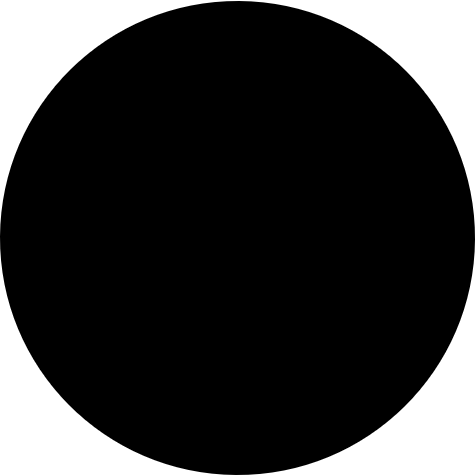
\includegraphics[scale=0.025]{Figs/circle_full.png}}
\newcommand{\circlehalf}{
\includegraphics[scale=0.025]{Figs/circle_half.png}}
\newcommand{\circleempty}{
\includegraphics[scale=0.025]{Figs/circle_empty.png}}
\begin{table*}
	\centering
	\begin{tabular}{|c|c|c|c|c|c|}

		\hline
		\diagbox[width=1.52in,height=0.4in] {\textbf{Defense}}{\textbf{Attack}} & \makecell*[c]{Facedancer~\cite{facedancer},\\ Syzkaller~\cite{syzkaller}} &\cite{rubber, badusb, rubberducky2020, usbbypassing, iseeyou, usbdriver} & JFC~\cite{JFC}&		\makecell{
			Duqu~\cite{duqu}, \\
			\cite{brain, stuxnet, conficker,flame}} & \tool \\
		\hline
		\makecell{USB condom~\cite{Condom}} & \makecell*[c]{\circlefull} & \circlefull & \circlefull &\circlefull& \circlefull\\
		\hline
		\makecell{
			Windows Defender ATP~\cite{windenfenderwhite}, \\
			Mohammadmoradi \emph{et al.}~\cite{mohammadmoradi2018making}, \\
			TMSUI~\cite{yang2015tmsui}
		}& \circleempty & \circlehalf & \circlehalf &\circlehalf& \circlehalf\\

		\hline
		\makecell{GoodUSB~\cite{tian2015defending}} & \makecell*[c]{\circlehalf} & \circlefull & \circlefull &\circlefull& \circleempty\\
		\hline

		\makecell{Neuner \emph{et al.}~\cite{neuner2018usblock}} & \makecell*[c]{\circleempty} & \circlefull & \circleempty &\circleempty& \circleempty\\
		\hline
		\makecell{Pham \emph{et al.}~\cite{pham2010optimizing}} & \makecell*[c]{\circleempty} & \circleempty & \circleempty &\circlefull& \circleempty\\
		\hline
		\makecell{JFCGuard~\cite{meng2018252}} & \makecell*[c]{\circleempty} & \circleempty & \circlehalf &\circleempty&   \circlehalf \\
			\hline
	\end{tabular}
	\linebreak
    \begin{tablenotes}
	\footnotesize
	\item[1] \circlefull  \@ means that the defense is effective
	\item[2] \circlehalf \@ means that the defense is partial effective
	\item[3] \circleempty \@  means that the defense is not effective
	\end{tablenotes}
	\caption{Effectiveness of Defenses against USB Attacks}
	\label{table:attack_vs_defense}
\end{table*}




